\documentclass{standalone}
\usepackage{tikz}
\usepackage{amsmath,dsfont,bm}
\usetikzlibrary{arrows.meta, positioning, shapes.geometric, calc,patterns,quotes,decorations.pathreplacing}
\newcommand \thetaQ {\bm{\theta}^{Q}}
\begin{document}
	
	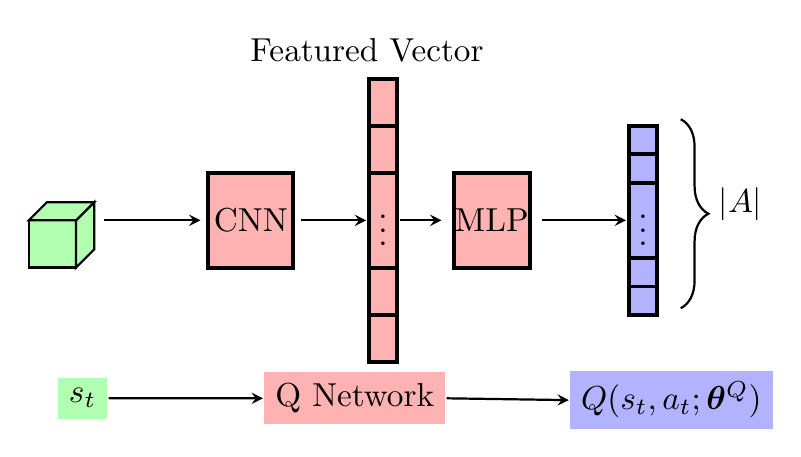
\begin{tikzpicture}[
		thick,scale=1.2, every node/.style={scale=1.2},
		state/.style={draw,circle,pattern=north east lines, pattern color=yellow,radius=0.2},
		action/.style={draw,rectangle, ,pattern=north west lines, pattern color=green}
		]
		
		% Input node (dashed ellipse)
		\pgfmathsetmacro{\cubex}{0.5}
		\pgfmathsetmacro{\cubey}{0.5}
		\pgfmathsetmacro{\cubez}{0.5}
		\draw[black,fill=green!30] (-2.4,0,0) -- ++(-\cubex,0,0) -- ++(0,-\cubey,0) -- ++(\cubex,0,0) -- cycle;
		\draw[black,fill=green!30] (-2.4,0,0) -- ++(0,0,-\cubez) -- ++(0,-\cubey,0) -- ++(0,0,\cubez) -- cycle;
		\draw[black,fill=green!30] (-2.4,0,0) -- ++(-\cubex,0,0) -- ++(0,0,-\cubez) -- ++(\cubex,0,0) -- cycle;
		
		
		% Hidden layers (rectangles)
		\draw[fill=red!30,line width=0.5mm] (-1,0.5) rectangle (-0.1,-0.5) node(CNN)[pos=.5] {CNN};
		\draw[fill=red!30,line width=0.5mm] (0.7,1.5) rectangle (0.9,-1.5) node[pos=-0.1] {Featured Vector} ;
		\foreach \y in {-1.5,-1.0,-0.5,0.5,1.0}
		\draw[fill=red!30,line width=0.5mm] (0.7,1.5) rectangle (1,\y) ;
		\node (FV) at (0.85, 0) {$\vdots$};
		\draw[fill=red!30,line width=0.5mm] (1.6,0.5) rectangle (2.4,-0.5) node(MLP)[pos = 0.5]{MLP};
		
		
		% Output vector
		\foreach \y in {-1.0, -0.7,-0.4,0.4, 0.7,1.0}
		\draw[fill=blue!30,line width=0.5mm] (3.45,1) rectangle (3.75,\y) ;
		\node (output) at (3.6, 0) {$\vdots$};
		
		
		% Arrows between layers
		\draw[->,>=stealth,thick] (-2.1,0) -- (CNN.west);
		\draw[->,>=stealth,thick] (CNN.east) -- (FV.west);
		\draw[->,>=stealth,thick] (FV.east) -- (MLP.west);
		\draw[->,>=stealth,thick] (MLP.east) -- (output.west);
		
		
		
		% Dotted line between layers
		%	\draw[dotted,thick] (0,0) -- (1,0);
		
		
		% Output arrows
		%	\foreach \y in {1.0, 0.5, -0.5, -1.0}
		%	\draw[->,>=stealth,thick] (3,0) -- (3.5,\y);
		
		% Output circles
		%	\foreach \y in {1.0, 0.5, -0.5, -1.0}
		%	\filldraw[fill=blue!30] (3.9,\y) circle [radius=0.2];
		
		% Output label
		\draw [thick, decorate,decoration={brace,amplitude=10pt},yshift=2pt] (4,1) -- (4,-1) node [black,midway,xshift = 18pt,yshift=3pt] {$|\mathds{A}|$};
		
		% Network label
		
		
		\node [fill = red!30!,below =of CNN,yshift = -5mm,xshift = 11mm](NN) {Q Network};
		\node [fill = green!30,left=of NN,xshift = -8mm] (st){$s_t$};
		
		% Q-function label
		\node [fill = blue!30,below = of output,yshift = -3.5mm,xshift = 3mm] (Q) { $Q(s_t,a_t;\thetaQ)$};
		\draw[->,>=stealth,thick](st)--(NN);
		\draw[->,>=stealth,thick](NN.east)--(Q.west);
	\end{tikzpicture}
	
\end{document}
